% =====================================================================
% AI Academy -- National AI Center
% Software Engineering Final Project -- Team Report
% Built from templates/REPORT_TEMPLATE.tex (preamble and section order kept;
% the guidance boxes were replaced by the answers).
%
% Compile with pdfLaTeX twice. The figure is read from ../docs/figures/; on
% Overleaf, upload docs/figures/architecture.pdf next to this file.
% Do not commit .aux/.log/.out/.toc files.
%
% HOW TO USE
% ----------
%   1. Edit the CONFIGURATION block below (team name, topic, members).
%   2. Replace every [TODO: ...] with your content. TODOs render in red,
%      so anything you forgot will be visually obvious in the PDF.
%   3. Three kinds of cues throughout:
%        - REQUIRED DELIVERABLE box (blue): exactly what we expect.
%        - PROBING QUESTIONS box (amber): NOT a checklist; these are
%          prompts that should shape how you write the section. A strong
%          response engages with at least 2 of them; a weak response
%          ignores them all.
%        - "Your response:" placeholders: replace with your text/diagram.
%   4. Target length: 8-10 pages including figures, excluding bibliography.
%   5. Compile with pdfLaTeX. Overleaf works out of the box.
% =====================================================================

\documentclass[11pt,a4paper]{article}

% ===== EARLY MACROS (must come before configuration) =================
% (Full styling lower down; we just need \TODO and \ph available
% before the configuration block uses them.)
\usepackage[dvipsnames]{xcolor}
\definecolor{accent2}{HTML}{8B0000}
\definecolor{ph}{HTML}{6B7280}
\newcommand{\TODO}[1]{\textcolor{accent2}{\textbf{[TODO: #1]}}}
\newcommand{\phh}[1]{\textcolor{ph}{\textit{#1}}}

% ===== CONFIGURATION (edit these) ====================================
\newcommand{\teamname}{Research Assistant Team}
\newcommand{\topicchoice}{Topic 4 -- Async Research Assistant}
\newcommand{\member}[2]{\textbf{#1} (#2)}  % name, GitHub handle
\newcommand{\reportdate}{\today}
\newcommand{\repolink}{\url{https://github.com/ruslan-sadigov/research-assistant-SWE-Final-Project}}

% ===== course meta (rarely changes) ==================================
\newcommand{\coursecode}{AI-ENG-110}
\newcommand{\coursename}{Software Engineering}
\newcommand{\institution}{AI Academy, National AI Center}
\newcommand{\semester}{Spring 2026}

% ===== PACKAGES ======================================================
\usepackage[margin=2.2cm,headheight=15pt]{geometry}
\usepackage[T1]{fontenc}
\usepackage[utf8]{inputenc}
\usepackage[final,protrusion=true,expansion=false]{microtype}
\usepackage{amsmath,amssymb}
\usepackage{graphicx}
\usepackage{booktabs}
\usepackage{array}
\usepackage{tabularx}
\usepackage{ragged2e}
\usepackage{enumitem}
\usepackage[parfill]{parskip}
\usepackage{listings}
\usepackage[most]{tcolorbox}
\usepackage{titlesec}
\usepackage{fancyhdr}
\usepackage{lastpage}
\usepackage[hidelinks]{hyperref}
\usepackage{xurl} % lets long URLs break
\graphicspath{{../docs/figures/}{./}}

\emergencystretch=3em
\hbadness=10000
\hfuzz=2pt

\hypersetup{
  colorlinks=true,
  linkcolor=NavyBlue,
  urlcolor=NavyBlue,
  citecolor=NavyBlue,
  pdftitle={\coursecode\ Final Project Report},
  pdfauthor={\teamname}
}

% ===== STYLING =======================================================
\definecolor{accent}{HTML}{0B3D91}
\definecolor{soft}{HTML}{F2F4F8}
\definecolor{deliver}{HTML}{E8F0FE}
\definecolor{deliverframe}{HTML}{1A56DB}
\definecolor{probe}{HTML}{FFF8E1}
\definecolor{probeframe}{HTML}{B45309}

\titleformat{\section}
  {\Large\bfseries\color{accent}}{\thesection.}{0.6em}{}
\titleformat{\subsection}
  {\large\bfseries\color{accent}}{\thesubsection}{0.5em}{}

\newcommand{\ans}[1]{\rule[-2pt]{#1}{0.5pt}}
\let\ph\phh  % alias the early \phh as \ph for consistency with the body

% Deliverable callout (light blue)
\newtcolorbox{deliverbox}{
  colback=deliver, colframe=deliverframe, boxrule=0.5pt,
  arc=2pt, left=8pt, right=8pt, top=4pt, bottom=4pt
}
% Probing-question callout (light amber)
\newtcolorbox{probebox}{
  colback=probe, colframe=probeframe, boxrule=0.5pt,
  arc=2pt, left=8pt, right=8pt, top=4pt, bottom=4pt
}

\newcommand{\answerbox}[1]{%
  \par\noindent
  \fcolorbox{black!30}{soft}{%
    \parbox{\dimexpr\linewidth-2\fboxsep-2\fboxrule\relax}{%
      \vspace{0pt}\centering
      \ph{[Your response here -- replace this placeholder.]}
      \vspace{#1}
    }%
  }\par
}

\newcommand{\figureplaceholder}[1]{%
  \par\noindent
  \begin{center}
  \fcolorbox{black!30}{soft}{%
    \parbox{0.75\linewidth}{%
      \vspace{0pt}\centering
      \ph{[Replace this box with \texttt{\textbackslash includegraphics\{...\}} or a tikzpicture.]}
      \vspace{#1}
    }%
  }
  \end{center}
}

\definecolor{codegreen}{rgb}{0,0.55,0}
\definecolor{codegray}{rgb}{0.4,0.4,0.4}
\definecolor{codepurple}{rgb}{0.55,0,0.78}
\definecolor{backcolour}{rgb}{0.97,0.97,0.97}

\lstdefinestyle{python}{
  language=Python,
  backgroundcolor=\color{backcolour},
  commentstyle=\color{codegreen},
  keywordstyle=\color{accent},
  numberstyle=\tiny\color{codegray},
  stringstyle=\color{codepurple},
  basicstyle=\ttfamily\footnotesize,
  breakatwhitespace=false,
  breaklines=true,
  keepspaces=true,
  numbers=left,
  numbersep=6pt,
  tabsize=2,
  frame=single,
  framerule=0.4pt,
  rulecolor=\color{black!30},
}

\pagestyle{fancy}
\fancyhf{}
\fancyhead[L]{\small\textit{\coursecode\ -- Final Report -- \teamname}}
\fancyhead[R]{\small\textit{\semester}}
\fancyfoot[L]{\small\textit{\institution}}
\fancyfoot[R]{\small Page \thepage\ of \pageref{LastPage}}
\renewcommand{\headrulewidth}{0.4pt}
\renewcommand{\footrulewidth}{0.4pt}

% =====================================================================
% ===== EVIDENCE VALUES (keep equal to the slides) =====================
\newcommand{\owntests}{267}
\newcommand{\smoketests}{16}
\newcommand{\alltests}{283}
\newcommand{\coveragepct}{98.44}
\newcommand{\imagesize}{218.67\,MB}
\newcommand{\cmd}[1]{\texttt{#1}}
\lstdefinestyle{plain}{
  basicstyle=\ttfamily\footnotesize,
  backgroundcolor=\color{backcolour},
  breaklines=true,
  columns=fullflexible,
  keepspaces=true,
  upquote=true,
  frame=single,
  framerule=0.4pt,
  rulecolor=\color{black!30},
}

\begin{document}

\begin{center}
{\small \textsc{\institution} \\[0.2em] \textsc{\coursecode\ -- \coursename\ -- \semester}}\\[1.2em]
{\Large\bfseries\color{accent} Final Project Report}\\[0.3em]
{\LARGE\bfseries \topicchoice}\\[0.6em]
\rule{0.85\textwidth}{0.6pt}
\end{center}

\vspace{0.6em}
\begin{tabularx}{\textwidth}{@{}lX@{}}
\textbf{Team:} & \teamname \hfill \textbf{Date:} \reportdate \\
\textbf{Repo:} & {\small\repolink} \hfill \textbf{Tag:} \texttt{v1.0-final} \\
\textbf{Members:} & \member{Ruslan Sadigov}{@ruslan-sadigov},\quad
  \member{Nihat Ismayilzade}{@NihatIsmayilzade},\newline
  \member{Samur Eyyubov}{@eyyubovsamur240-afk},\quad
  \member{Polad Ibrahimli}{@Polad-Ibrahimli} \\
\end{tabularx}
\vspace{0.4em}\hrule\vspace{0.6em}

% ===== EXECUTIVE SUMMARY =============================================
\section*{Executive Summary}
\addcontentsline{toc}{section}{Executive Summary}

We built an asynchronous research assistant: a command-line tool that takes a
question, collects evidence from Wikipedia, arXiv and a web-search provider at
the same time, and asks an LLM for an answer whose numbered citations point to
that evidence. Around the unchanged instructor-supplied \texttt{ai/} package we
added validated configuration, a concurrency layer with one deadline per source,
bounded retries with arXiv request pacing, a SQLite evidence cache, structured
logging, \owntests{} tests of our own at \coveragepct\,\% coverage, and a
multi-stage Docker image of \imagesize{}. In a controlled offline benchmark over
the five supplied questions, concurrent collection took 0.31\,s against 0.62\,s
sequentially, the ideal 2.0$\times$ for our source delays; against the live
services it was faster for four of the five questions (0.79--1.82$\times$). Our
headline robustness case is a live run in which arXiv timed out: the user still
received an answer built from Wikipedia's evidence, with a warning naming arXiv.
The most surprising lesson was how much the supplied fetchers depend on the
surrounding layer: called directly, Wikipedia rejected them (HTTP 403, no
User-Agent) and arXiv answered with a redirect, and full-sentence questions find
nothing in Wikipedia search. Starting again, we would rewrite questions into
short topic queries and put provider settings into the cache key from day one.

\tableofcontents
\vspace{0.6em}\hrule\vspace{0.4em}

% =====================================================================
\section{Project Overview}

\subsection{Problem framing \& scope}

A user wants a quick, sourced answer to a research question without opening
three websites. The system accepts the question and a selection of sources,
retrieves evidence from each selected source concurrently, and prints an answer
in which every bracketed number refers to a listed reference. A source that
fails or times out must not take the others down: the answer is produced from
whatever evidence arrived, and the failure is reported as a warning.

\textbf{Inputs:} the question (at most \cmd{MAX\_QUESTION\_LENGTH} = 2000
characters after trimming), \cmd{-{}-sources} with any of \cmd{wiki},
\cmd{arxiv}, \cmd{web}, an optional \cmd{-{}-no-cache} flag, and settings from
environment variables or \cmd{.env}. \textbf{Outputs:} the answer, numbered
references, per-source warnings, and an exit code (0 answer produced, 1 no
answer, 2 invalid input or configuration); retrieved evidence is cached in
SQLite for 24\,hours. \textbf{Entry point:} one CLI command,
\cmd{python -m researcher ask "<question>" -{}-sources wiki,arxiv,web}, also the
entry point of the Docker runtime image.

\textbf{Scope decisions.} We deliberately built no HTTP API or UI: a single-user
CLI met the topic, and every added entry point would need its own validation and
tests. We tightened the specification by validating every input before any
network call, escaping control characters in all printed provider text, and
treating an empty result as a valid outcome rather than an error. We loosened it
in one place: we do not rewrite questions into search keywords, so Wikipedia
often returns nothing for full questions (Section~\ref{sec:limits}).

\subsection{Provider choice and the AI module contract}

\begin{center}\small
\begin{tabularx}{\textwidth}{@{}llX@{}}
\toprule
\textbf{Role} & \textbf{Provider} & \textbf{Identifier / setting} \\
\midrule
LLM (synthesis) & Google Gemini (\texttt{google-genai} SDK) & \cmd{LLM\_PROVIDER=gemini}\newline\cmd{LLM\_MODEL=gemini-3.5-flash-lite} \\
Web search & Tavily & \cmd{WEB\_SEARCH\_PROVIDER=tavily} \\
Encyclopedia & Wikipedia search API & no key \\
Papers & arXiv export API & no key \\
Embeddings & not used & -- \\
\bottomrule
\end{tabularx}
\end{center}

Only \texttt{AIService} calls the supplied package: \cmd{ai.fetch\_wikipedia},
\cmd{ai.fetch\_arxiv} and \cmd{ai.fetch\_web} (each with \cmd{client=} and
\cmd{max\_results=}), and \cmd{ai.synthesize}. Other modules only use its data
types \cmd{Source}, \cmd{Citation} and \cmd{AnswerWithCitations}, and
\cmd{ProviderError} for error classification. \emph{We did not modify the public
interface, or any file, of the provided \texttt{ai/} package.}

\textbf{Malformed responses.} The supplied synthesizer already drops citation
indices that do not refer to a provided source. Our layer adds three checks:
arXiv responses whose entries point to arXiv's \cmd{/api/errors} feed are
rejected as a provider error, because the supplied parser would otherwise
return an error message as a ``paper'' and we would cache it; every application
model rejects unknown fields and enforces invariants (an \cmd{ok} outcome must
contain sources, a failed or timed-out one must carry a warning and cannot be a
cache hit); and cached rows are re-validated on every read. What we cannot
detect is a well-formed answer that is wrong: citations show which evidence was
used, not that the answer is true.

% =====================================================================
\section{Architecture}\label{sec:arch}

\subsection{Module map}

\begin{figure}[h]
\centering
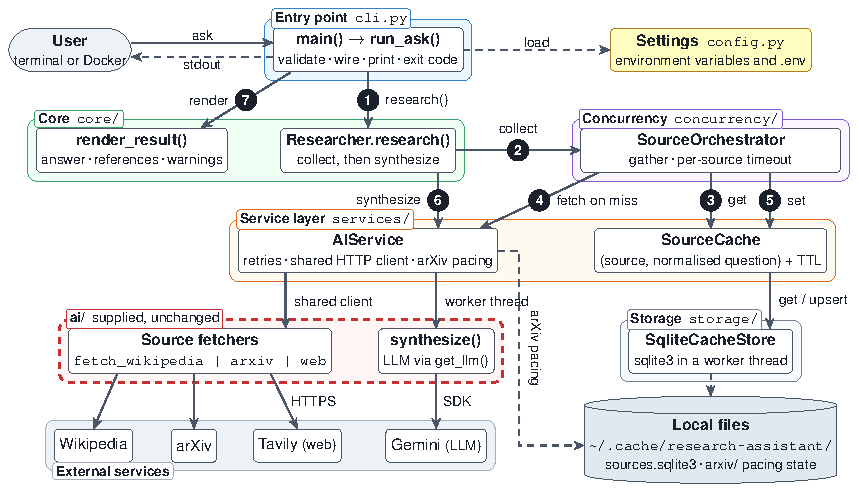
\includegraphics[width=\textwidth]{architecture.pdf}
\caption{Runtime architecture of one \cmd{ask} request. Solid arrows are calls
from caller to callee, numbered in request order; dashed arrows are
configuration, local files or output. Tab paths are relative to
\cmd{src/researcher/}. Source: \cmd{docs/figures/architecture.tex}.}
\label{fig:arch}
\end{figure}

The \textbf{entry point} (\cmd{cli.py}) validates input and is the only place
that wires concrete classes. The \textbf{core} (\cmd{core/researcher.py}) first
collects evidence, then synthesizes, and turns missing evidence or a failed
synthesis into warnings. The \textbf{concurrency layer}
(\cmd{concurrency/orchestrator.py}) runs the selected sources together, each
under its own deadline, and performs the cache-read, fetch and cache-write
sequence. The \textbf{service layer} wraps the supplied package
(\cmd{services/ai\_service.py}, with arXiv pacing in \cmd{arxiv\_limit.py}) and
owns cache keys and expiry (\cmd{services/cache.py}). The \textbf{storage layer}
(\cmd{storage/cache\_store.py}) only reads and writes rows.

\textbf{Interpreting the diagram.} Two arrows cross the \texttt{ai/} boundary,
both from \texttt{AIService}; the shared HTTP client also crosses it in the other
direction as the \cmd{client=} argument, so the supplied fetchers send their
requests through our retrying transport, User-Agent header and redirect
handling. Only \texttt{SourceCache} crosses into storage, through
\cmd{CacheStoreProtocol}; \texttt{AIService} also writes arXiv pacing files.
Swapping Gemini for OpenAI or Anthropic changes \emph{no Python file}: provider
selection lives inside \texttt{ai/} and reads \cmd{LLM\_PROVIDER}. It changes
\cmd{.env} and adds the SDK to \cmd{pyproject.toml} and \cmd{uv.lock}.

\subsection{OOP design \& key abstractions}

We chose composition with \texttt{typing.Protocol} interfaces over abstract base
classes. Components receive collaborators through their constructors, and
\cmd{run\_ask()} in \cmd{cli.py} wires them:

\begin{lstlisting}[style=python]
# src/researcher/cli.py -- run_ask()
ai_service = AIService(settings)
cache = SourceCache(store, settings.cache_ttl_seconds)
orchestrator = SourceOrchestrator(settings, ai_service, cache)
researcher = Researcher(orchestrator, ai_service)
result = await researcher.research(question, sources, use_cache=use_cache)

# src/researcher/interfaces.py
class CacheStoreProtocol(Protocol):
    async def get_entry(
        self, source: SourceName, query_key: str
    ) -> CacheEntry | None: ...
    async def upsert_entry(self, entry: CacheEntry) -> None: ...
\end{lstlisting}

\textbf{Why Protocols rather than ABCs.} The parts vary independently: two
stores (\texttt{SqliteCacheStore} and \texttt{InMemoryCacheStore}) sit behind one
\texttt{SourceCache}, and the tests replace the AI service, cache and store with
small fakes that satisfy the protocols structurally, without inheriting from
anything or patching modules; mypy still checks the signatures. An ABC would add
a base class to every fake for no runtime benefit, and a plain callable would not
cover multi-method objects such as a store. Inheritance appears only where a
framework expects it: Pydantic models and settings, exceptions
(\texttt{HTTPRetryExhausted} extends the supplied \texttt{ProviderError}, so
callers still see a provider error), and \texttt{RetryingTransport}, which
subclasses \texttt{httpx.AsyncBaseTransport} but \emph{wraps} the real transport
by composition, so retries apply to any transport, including test mocks.

\subsection{Data flow across module boundaries}

Our own boundary types are Pydantic models rather than dataclasses, because they
validate on construction: \texttt{Settings}, \texttt{SourceOutcome} (source,
status \cmd{ok}/\cmd{empty}/\cmd{failed}/\cmd{timeout}, sources, elapsed time,
\cmd{cache\_hit}, warning), \texttt{CollectionResult} (outcomes, de-duplicated
sources, elapsed time), \texttt{ResearchResult} (question, collection, answer,
warnings) and \texttt{CacheEntry} (source, normalised key, sources,
\cmd{created\_at}, \cmd{expires\_at}); \cmd{SourceName} and \cmd{SourceStatus}
are \texttt{Literal} types. \emph{No naked dictionaries cross module boundaries};
the only JSON is the serialized \texttt{CacheEntry} inside the SQLite store.

We reused \cmd{ai.Source} and \cmd{ai.AnswerWithCitations} unchanged, because
they already describe evidence and answers. We wrapped them when a layer needed
information the supplied types cannot carry: per-source status, timing, cache
hits and warnings (\texttt{SourceOutcome}), and persistence metadata
(\texttt{CacheEntry}).

% =====================================================================
\section{Concurrency \& Performance}\label{sec:concurrency}

\subsection{Why this concurrency model}

The work is almost entirely waiting on network I/O, so we use \texttt{asyncio}:
\texttt{SourceOrchestrator} starts one task per unique selected source with
\cmd{asyncio.gather}, and each task runs inside \cmd{asyncio.timeout}
(\cmd{PER\_SOURCE\_TIMEOUT\_SECONDS}, default 10\,s), which covers its cache read,
fetch attempts, retry waits, arXiv pacing and cache write. The bottleneck we
target is the sum of source latencies: sequentially a question waits for every
source in turn, concurrently only for the slowest. The \textbf{bound} is
structural: at most one task per source, so three per question; no semaphore is
needed. Each task catches its own failures and returns an outcome, which is why
we use \cmd{gather} rather than \texttt{TaskGroup} (which cancels siblings on the
first error). Blocking work leaves the event loop through
\cmd{asyncio.to\_thread}: SQLite operations and \cmd{ai.synthesize}.

Threads would also work for three I/O calls, but asyncio gives us one shared
HTTP client, cancellable deadlines and deterministic tests without locks around
shared state. Concurrency pays off as soon as two sources are selected, since
their waits overlap. A semaphore of 1 would make the design sequential; a
semaphore of 100 would change nothing, because there are never more than three
tasks.

\subsection{Sequential-vs-concurrent benchmark}

\textbf{Offline} (\cmd{benchmarks/benchmark\_sources.py}): the real orchestrator
with simulated source delays of 0.1, 0.2 and 0.3\,s, one warm-up excluded, median
of five alternating runs; recorded 2026-09-16 on Windows~11 (AMD64), Python
3.12.11. \textbf{Live} (\cmd{benchmarks/benchmark\_live\_sources.py}): real
Wikipedia, arXiv and Tavily requests, one measured pair per question, 3.1\,s pause
before each collection; recorded 2026-09-16 on Windows, Python 3.12.11. Both use
the five supplied questions with all three sources ($N = 3$ requests per
question, 15 per mode) and \emph{no cache}; synthesis is excluded.

\begin{center}\small
\begin{tabular}{llcccc}
\toprule
\textbf{Mode} & \textbf{Workload} & $N$ & \textbf{Sequential (s)} & \textbf{Concurrent (s)} & \textbf{Speedup} \\
\midrule
Offline & q1 Photosynthesis & 3 & 0.6282 & 0.3144 & 2.00$\times$ \\
Offline & q2 Long context windows & 3 & 0.6238 & 0.3126 & 2.00$\times$ \\
Offline & q3 Financial crisis & 3 & 0.6227 & 0.3135 & 1.99$\times$ \\
Offline & q4 Fusion energy & 3 & 0.6239 & 0.3133 & 1.99$\times$ \\
Offline & q5 CRISPR-Cas9 & 3 & 0.6226 & 0.3117 & 2.00$\times$ \\
\midrule
Live & q1 Photosynthesis & 3 & 6.009 & 3.616 & 1.66$\times$ \\
Live & q2 Long context windows & 3 & 4.411 & 5.596 & 0.79$\times$ \\
Live & q3 Financial crisis & 3 & 6.521 & 3.624 & 1.80$\times$ \\
Live & q4 Fusion energy & 3 & 4.550 & 4.343 & 1.05$\times$ \\
Live & q5 CRISPR-Cas9 & 3 & 7.044 & 3.868 & 1.82$\times$ \\
\bottomrule
\end{tabular}
\end{center}

\textbf{Interpretation.} $N\times$ is not the right ceiling here: with unequal
delays the ideal is \emph{sum/maximum} $= 0.6/0.3 = 2\times$, which the offline
run reaches within scheduling overhead. Live, every run returned the same
outcome (Wikipedia empty, three arXiv and three Tavily results, six unique URLs,
identical in both modes, no failures or timeouts). Concurrency won four of five
pairs; q2 was slower, and a single pair cannot tell whether network variance,
provider caching or arXiv's pacing caused it. The bottleneck is network latency
and arXiv's 3\,s request spacing, not the GIL or the database (the cache was off).
Going further would mean running several questions at once or rephrasing
queries, not adding workers.

\subsection{Rate limit \& politeness}

Two mechanisms apply. (1) \textbf{Sleep on retryable errors:} HTTP 408, 429 and
5xx, transport errors and timeouts are retried up to \cmd{RETRY\_MAX\_ATTEMPTS} = 3
attempts in total, waiting 0.5\,s, then 1\,s, doubling up to
\cmd{RETRY\_MAX\_DELAY\_SECONDS} = 4\,s, or longer when the server sends
\texttt{Retry-After}. (2) \textbf{arXiv pacing:} following arXiv's terms of
use~\ref{arxiv}, a file lock under \cmd{\textasciitilde/.cache/research-assistant/arxiv/}
serialises arXiv requests across processes and leaves at least 3\,s after the
previous request completed; a \texttt{Retry-After} from arXiv is stored as a
cooldown for all processes. Wikipedia requests carry a descriptive User-Agent, as
its policy requires~\ref{wikiua}.

The offline test suite makes no real provider calls; its largest burst is three
simulated source calls per question. We have not observed an HTTP 429 from a live
provider; the path is exercised with mocked 408, 429, 500 and 503 responses. We
did observe intermittent Gemini 503 (``high demand'') responses, which take the
same retry path and are logged as, for example,
\cmd{AI operation failed: operation=synthesis attempt=1 max\_attempts=3
error\_type=... http\_status=503}.

% =====================================================================
\section{Robustness \& Error Handling}\label{sec:robustness}

\subsection{Wrapping the AI module}

\textbf{Retries.} Retryable: HTTP 408/429/5xx, \texttt{httpx} transport errors,
timeouts, connection errors and SDK connection or timeout errors. Not retried:
other 4xx, invalid values, missing packages, too many redirects, and supplied
\cmd{ProviderError}s that signal setup problems (a key ``is not set'', an unknown
provider, malformed XML). HTTP requests are retried inside the transport; when
that budget is exhausted it raises \texttt{HTTPRetryExhausted}, which the outer
fetch retry does not repeat, so one source never makes $3\times3$ requests.
\textbf{Timeouts.} The HTTP client uses the per-source value, and the
orchestrator's \cmd{asyncio.timeout} bounds the whole source. Synthesis has no
separate deadline: its attempts are bounded by the retry settings, and an SDK call
already running in a worker thread cannot be cancelled. \textbf{Logging.} Every
failed attempt logs \cmd{operation}, \cmd{attempt}, \cmd{max\_attempts},
\cmd{error\_type} and \cmd{http\_status} at WARNING; each source logs
\cmd{source}, \cmd{status}, \cmd{cache\_hit}, \cmd{results} and
\cmd{elapsed\_seconds} at INFO; timeouts log \cmd{source}, \cmd{stage} and
\cmd{deadline\_expired}. Our own records never contain exception messages,
headers or keys; library loggers such as httpx still record request URLs at
INFO. \textbf{Validation} is described in Section~\ref{sec:validation}.

\textbf{Walk-through: HTTP 429 from Tavily.} The transport sees 429 and raises;
the retry waits the larger of 0.5\,s and \texttt{Retry-After}; a 200 on the
second attempt returns results as if nothing happened. If all three attempts
fail, the web source ends as \cmd{failed} with the warning ``web could not
retrieve evidence.'', while Wikipedia and arXiv evidence is still used.

\subsection{Failure-mode analysis (one concrete incident)}

\textbf{(i) Injection.} We pointed \cmd{DATABASE\_URL} at a file containing
plain text instead of a SQLite database and ran the real CLI for q1 with all
three sources (\cmd{tests/cache\_verification.py}; providers simulated, network
blocked).
\textbf{(ii) System behaviour.} For each source, the cache read raised
\texttt{CacheStoreError}; the orchestrator logged it, fetched fresh evidence,
tried to save it, failed again, and kept the evidence. Synthesis ran and the exit
code was 0. The file was left byte-for-byte unchanged.
\textbf{(iii) What the user saw:} the normal answer and references, followed by

\begin{lstlisting}[style=plain]
Warnings:
  - wiki cache could not be read; fetching fresh evidence. wiki results could not be saved to cache.
  - arxiv cache could not be read; fetching fresh evidence. arxiv results could not be saved to cache.
  - web cache could not be read; fetching fresh evidence. web results could not be saved to cache.
\end{lstlisting}

\textbf{(iv) Logs} (timestamps removed):

\begin{lstlisting}[style=plain]
WARNING researcher.concurrency.orchestrator: cache read failed: source=wiki; attempting fresh fetch
WARNING researcher.concurrency.orchestrator: cache write failed: source=wiki; fetched evidence retained
INFO researcher.concurrency.orchestrator: source completed: source=wiki status=ok cache_hit=False results=1 elapsed_seconds=0.002
\end{lstlisting}

A natural assumption is that a broken file is detected once per run; in fact
every read and write retries opening the file, so each run produces two warnings per source until
the file is removed. The logs name the source and stage but, deliberately, not the
path, so diagnosing requires checking \cmd{DATABASE\_URL}. We documented the
missing repair as a finding rather than changing the working cache code. The same
degradation happened in a \textbf{live} run where arXiv hit its deadline: the
answer was built from Wikipedia's evidence and printed with an arXiv warning
(reproduced offline by \cmd{test\_deadline\_cancels\_slow\_fetch\_and\_preserves\_success}).

\subsection{Input validation}\label{sec:validation}

\begin{center}\small
\begin{tabularx}{\textwidth}{@{}lXX@{}}
\toprule
\textbf{Entry} & \textbf{Rule} & \textbf{User message (exit code 2)} \\
\midrule
Question & Trimmed; not empty; at most \cmd{MAX\_QUESTION\_LENGTH} characters &
\cmd{Invalid input: Question must not be empty.} / \cmd{... Question is N characters, which exceeds the maximum of 2000.} \\
\cmd{-{}-sources} & Comma list, case-insensitive, known names only, duplicates removed, at least one &
\cmd{Invalid input: Unknown source(s): x. Valid: wiki, arxiv, web} / \cmd{Select at least one source.} \\
Environment & Typed and range-checked (positive, finite, max delay $\ge$ initial delay, known log level); values never echoed &
\cmd{Invalid configuration; check environment settings and the .env file.} \\
\cmd{DATABASE\_URL} & \cmd{sqlite:///} plus a file path; no \cmd{:memory:}, \cmd{?}, \cmd{\#} or NUL &
\cmd{Invalid cache configuration; DATABASE\_URL must be a SQLite file URL.} \\
Output & Control and formatting characters in provider text are escaped before printing & -- \\
\bottomrule
\end{tabularx}
\end{center}

A 50{,}000-character question is rejected before any network call. There is no
file or image input. \cmd{DATABASE\_URL} may point anywhere the user can write:
it is operator configuration on the user's own machine, not remote input.

% =====================================================================
\section{Storage \& Caching}\label{sec:storage}

\subsection{Schema}

Read back from a database the application created
(\cmd{PRAGMA user\_version = 1}, rollback-journal mode):

\begin{lstlisting}[style=python,language=sql,numbers=none,basicstyle=\ttfamily\small]
CREATE TABLE cache_entries (
    source TEXT NOT NULL,        -- 'wiki' | 'arxiv' | 'web'
    query_key TEXT NOT NULL,     -- question after normalize_query()
    payload TEXT NOT NULL,       -- whole CacheEntry as JSON
    PRIMARY KEY (source, query_key)
);
-- index sqlite_autoindex_cache_entries_1: unique, created for the primary key
\end{lstlisting}

The composite primary key's automatic unique index is the only index; it serves
the only query the store runs (\cmd{WHERE source = ? AND query\_key = ?}) and turns
a repeated write into an in-place update. There are \textbf{no foreign keys},
because there is one table. \textbf{Every column is derived}: rows are copies of
what the external services returned at fetch time, and those services remain the
source of truth, so deleting the file costs speed and API quota, not
information. \cmd{query\_key} is derived from the question, and
\cmd{created\_at}/\cmd{expires\_at} inside the payload are cache metadata. We store
the entry as JSON rather than normalised columns because it is always read and
written whole and validated by \cmd{CacheEntry} on read; the price is that expiry
is invisible to SQL. \cmd{tests/test\_cache\_store\_contract.py} fails if this
layout changes.

\subsection{Caching policy}

\textbf{What:} source evidence per (source, normalised question); answers are
never cached, so every run synthesizes. \textbf{Key normalisation:} Unicode NFKC,
collapsed whitespace, trailing \texttt{?!.} removed, case-folded.
\textbf{How long:} \cmd{CACHE\_TTL\_SECONDS} = 86\,400 (24\,h); an entry is a miss
from its expiry second. Empty results are cached too; failures and timeouts are
not. \textbf{Where:} \cmd{\textasciitilde/.cache/research-assistant/sources.sqlite3}
by default, or \cmd{DATABASE\_URL}; in Docker, a named volume at
\cmd{/home/appuser/.cache/research-assistant}. \cmd{-{}-no-cache} never opens the
file. \textbf{Invalidation:} expiry only; an expired row is replaced by the next
successful fetch of the same key; otherwise delete the file or change
\cmd{DATABASE\_URL}.

\textbf{Hit rate} (hits / eligible lookups), measured by
\cmd{tests/cache\_verification.py} through the real CLI with simulated providers,
five questions $\times$ three sources: \textbf{0/15 on the first run, 15/15 on the
second, 15/30 = 50\,\% combined}; all ten runs still synthesized an answer.
Reformatted questions (other case, spacing and trailing punctuation) also hit
15/15, and a \cmd{-{}-no-cache} pass made no lookups and left the file unchanged.
Live, a repeated arXiv query reported \cmd{cache\_hit=True}, and CI shows a cache
hit across two separate containers sharing a volume.

\textbf{Staleness.} Three kinds of entry can mislead: an empty Wikipedia result
stays empty for 24\,h, entries fetched under another \cmd{WEB\_SEARCH\_PROVIDER} or
\cmd{MAX\_SOURCES\_PER\_QUERY} are served because the key ignores settings, and
sources can change within the TTL. In production we would add a settings
fingerprint to the key, a shorter TTL for empty results, an indexed
\cmd{expires\_at} column with a purge command, and a size bound.

% =====================================================================
\section{Testing}\label{sec:testing}

\subsection{Strategy \& coverage}

\begin{center}\small
\begin{tabular}{lc}
\toprule
\textbf{Suite} & \textbf{Result} \\
\midrule
\texttt{src/researcher} (our SE layer), \owntests{} tests & \coveragepct\,\% line coverage \\
Provided \texttt{ai/} smoke tests (\smoketests{}) & passing \\
Ruff, Black, isort, mypy (15 source files) & clean \\
\bottomrule
\end{tabular}
\end{center}

All \alltests{} tests run offline (\cmd{uv run python -m pytest -{}-cov=researcher}).
We mock at two levels: fakes that satisfy \cmd{AIServiceProtocol} or the cache
protocols, and replacements for the \cmd{ai.fetch\_*} and \cmd{ai.synthesize}
functions so the real CLI, service, orchestrator and SQLite store still run. HTTP
behaviour is tested with \cmd{httpx.MockTransport}; network sends are blocked
elsewhere, so the suite makes no real provider calls. CI runs lint, type checks
and tests, builds the Docker test image, runs it with \cmd{-{}-network none}, and
checks the cache across two runtime containers.

\textbf{Not covered, on purpose:} the \cmd{\_\_main\_\_.py} shim and the
\cmd{if \_\_name\_\_ == "\_\_main\_\_"} line, the file-locking branch for the
\emph{other} operating system in \cmd{arxiv\_limit.py} (each platform runs only
its own), two rarely reached branches in \cmd{ai\_service.py} (an SDK
connection-error check and a final assertion) and one validator branch in
\cmd{config.py}. A weakness we accept: some store tests still inspect private
attributes (the SQLite connection), which ties them to implementation details.

\subsection{Notable tests}

\begin{enumerate}[leftmargin=*,itemsep=2pt]
\item \textbf{Happy path, end to end:} \cmd{tests/test\_sample\_questions.py} runs
  the real CLI three times for each supplied question (10 cases: all sources and
  each question's expected subset): first retrieval, SQLite reuse, then
  \cmd{-{}-no-cache}, checking exit codes, answers, references and fetch counts.
\item \textbf{Concurrency:} \cmd{test\_source\_failure\_preserves\_other\_evidence}
  makes arXiv raise \texttt{RuntimeError} or \texttt{TimeoutError} inside
  \cmd{gather}; the outcomes are \cmd{ok}, \cmd{failed}, \cmd{ok}, Wikipedia and
  web evidence is kept in order, and the shared client is closed. A companion
  test proves the fetches overlap and share one client.
\item \textbf{Error path with a real bug:}
  \cmd{test\_arxiv\_error\_feed\_rejected\_without\_retry} feeds an arXiv Atom error
  feed. The supplied parser returns it as an ordinary ``paper'', which we would
  have cached and cited; the service now rejects it without retrying. The HTTP
  retry test (\cmd{test\_http\_retries\_and\_closes\_responses}, statuses 408, 429,
  500, 503) also checks that every response is closed.
\end{enumerate}

\textbf{What we did not test:} scheduled live contract tests against the real
providers, and many CLI processes sharing one arXiv lock and one SQLite file
under load.

% =====================================================================
\section{Deployment \& Reproducibility}\label{sec:deploy}

\subsection{Docker image}

A \textbf{multi-stage} build on \cmd{python:3.12-slim} (Python 3.12.14 at
verification): a \cmd{builder} stage installs the locked dependencies with uv, a
\cmd{test} stage adds development tools and tests, and the \cmd{runtime} stage
copies only the installed environment and runs as non-root \cmd{appuser}
(UID 1000). The runtime image is \textbf{\imagesize{}} (218\,667\,271 bytes), below
the 250\,MB bonus limit; the test image is 569.65\,MB. uv, pytest, demo files and
\cmd{.env} are absent from the runtime image.

\begin{lstlisting}[style=plain]
docker build --target test -t research-assistant:test .
docker build --target runtime -t research-assistant:runtime .
docker run --rm --network none research-assistant:test
docker run --rm --env-file .env research-assistant:runtime `
  ask "Photovoltaic effect" --sources wiki,arxiv,web --no-cache
docker volume create research-assistant-cache
docker run --rm --env-file .env --env DATABASE_URL= `
  --mount type=volume,source=research-assistant-cache,target=/home/appuser/.cache/research-assistant `
  research-assistant:runtime ask "Photovoltaic effect" --sources wiki
\end{lstlisting}

The base is Debian \emph{slim} (glibc) rather than Alpine (musl), so the
prebuilt wheels resolved in \cmd{uv.lock} install without compilation.
Compared with the bare slim base ($\sim$120\,MB), the installed environment adds
roughly 100\,MB. In a live
container run, the three sources took 2.39, 3.53 and 0.53\,s, and collection
finished in 3.64\,s.

\subsection{Configuration}

Existing environment variables override \cmd{.env}; application settings with
invalid values stop the CLI with exit code 2.

\begin{center}\small
\begin{tabularx}{\textwidth}{@{}>{\raggedright\arraybackslash}p{0.43\textwidth}X@{}}
\toprule
\textbf{Variable (default)} & \textbf{Effect when missing} \\
\midrule
\cmd{LLM\_PROVIDER} (\cmd{gemini} in \cmd{.env.example}) & The supplied factory falls back to \cmd{anthropic}; without its key or SDK, synthesis fails: evidence is printed, exit code 1. \\
\cmd{LLM\_MODEL} & The provider's built-in default model. \\
\cmd{GOOGLE\_API\_KEY}\newline (or \cmd{GEMINI\_API\_KEY}, \cmd{LLM\_API\_KEY}) & Synthesis fails without retrying (``is not set''); evidence is still printed, exit code 1. \\
\cmd{WEB\_SEARCH\_PROVIDER} (\cmd{tavily}) & Tavily is used. \\
\cmd{TAVILY\_API\_KEY} & The web source fails at once with a warning; other sources continue. \\
\cmd{LOG\_LEVEL} (INFO)\newline \cmd{MAX\_QUESTION\_LENGTH} (2000)\newline
\cmd{PER\_SOURCE\_TIMEOUT\_SECONDS} (10)\newline \cmd{MAX\_SOURCES\_PER\_QUERY} (3)\newline
\cmd{RETRY\_MAX\_ATTEMPTS} (3)\newline \cmd{RETRY\_INITIAL\_DELAY\_SECONDS} (0.5)\newline
\cmd{RETRY\_MAX\_DELAY\_SECONDS} (4)\newline \cmd{CACHE\_TTL\_SECONDS} (86400)
& The default in brackets applies. \\
\cmd{DATABASE\_URL} (blank) & \cmd{\textasciitilde/.cache/research-assistant/sources.sqlite3}. \\
\bottomrule
\end{tabularx}
\end{center}

% =====================================================================
\section{Limitations \& Future Work}\label{sec:limits}

\begin{itemize}[leftmargin=*,itemsep=2pt]
\item \textbf{Wikipedia and full questions.} Live runs of the five supplied
  questions returned no Wikipedia matches; short topic queries such as
  ``Photovoltaic effect'' worked. With another week we would extract a topic query
  first.
\item \textbf{Single LLM, no fallback.} A Gemini outage or quota limit means
  evidence without an answer. Productionising would need a second provider and
  quota monitoring.
\item \textbf{Cache freshness.} Our weakest design decision: the key ignores
  provider settings, empty results live for the full TTL, and nothing evicts old
  rows (Section~\ref{sec:storage}).
\item \textbf{Untested under load.} Many processes sharing arXiv pacing will queue
  behind the 3\,s spacing and can hit their 10\,s deadlines; SQLite serialises
  writers. On a busy day, provider rate limits and this queue are the most likely
  breakage.
\item \textbf{Thin live evidence.} The live speedup rests on one pair per
  question; we would repeat it at least three times and compare distributions.
\end{itemize}

% =====================================================================
\section{Tools \& Acknowledgements}\label{sec:tools}

\textbf{AI assistance.} Samur Eyyubov used Claude (Anthropic) to draft the
architecture figure, the cache verification script
(\cmd{tests/cache\_verification.py}) and the three new
\cmd{tests/test\_cache\_*.py} files, the architecture and cache-verification
documents, the presentation, and the first draft of this report; he reviewed
the drafts against the repository before committing them. Each member's AI use
in their own modules is listed in the signed contribution statement.

\textbf{Acknowledgements.} The \texttt{ai/} package, sample questions, demo and
smoke tests were supplied by the course. We build on httpx, Pydantic,
pydantic-settings, python-dotenv, pytest (with pytest-asyncio and pytest-cov),
Ruff, Black, isort, mypy, uv and Docker.

% =====================================================================
\section*{References}
\addcontentsline{toc}{section}{References}
\begin{enumerate}[label={[\arabic*]},leftmargin=2.4em,itemsep=2pt]
  \item Python documentation, ``Coroutines and Tasks'' (\cmd{gather}, \cmd{timeout}, \cmd{to\_thread}), \url{https://docs.python.org/3/library/asyncio-task.html}
  \item HTTPX documentation, transports and clients, \url{https://www.python-httpx.org/}
  \item Pydantic and pydantic-settings documentation, \url{https://docs.pydantic.dev/}
  \item \phantomsection\label{arxiv}arXiv API Terms of Use (one request every three seconds), \url{https://info.arxiv.org/help/api/tou.html}
  \item \phantomsection\label{wikiua}Wikimedia User-Agent policy, \url{https://foundation.wikimedia.org/wiki/Policy:User-Agent_policy}
  \item RFC 9110, HTTP Semantics, \texttt{Retry-After}, \url{https://www.rfc-editor.org/rfc/rfc9110}
  \item SQLite documentation, PRAGMA statements, \url{https://www.sqlite.org/pragma.html}
  \item Tavily API documentation, \url{https://docs.tavily.com/}
  \item Google Gemini API documentation, \url{https://ai.google.dev/gemini-api/docs}
  \item Docker documentation, multi-stage builds, \url{https://docs.docker.com/build/building/multi-stage/}
\end{enumerate}

\appendix
% =====================================================================
\section{Appendix --- Reproducing the benchmark}

From a clone of the repository with uv installed (PowerShell). The offline
commands need no keys; the live benchmark needs \cmd{TAVILY\_API\_KEY} in
\cmd{.env} and consumes web-search quota.

\begin{lstlisting}[style=plain]
git clone https://github.com/ruslan-sadigov/research-assistant-SWE-Final-Project.git
cd research-assistant-SWE-Final-Project
uv sync --locked
uv run python benchmarks/benchmark_sources.py --repeats 5       # offline table
Copy-Item .env.example .env                                     # then add keys
uv run python benchmarks/benchmark_live_sources.py --repeats 1  # live table
uv run python tests/cache_verification.py                       # cache hit rate
uv run python -m pytest --cov=researcher --cov-report=term-missing
uv run python -m researcher ask "Photovoltaic effect" --sources wiki,arxiv,web
\end{lstlisting}

The same checks run in Docker with the commands in Section~\ref{sec:deploy}.
Methods and raw data: \cmd{docs/concurrency-benchmark.md},
\cmd{docs/live-benchmark.md}, \cmd{docs/cache-verification.md} and
\cmd{docs/docker.md}.

\vspace{1em}\hrule\vspace{0.6em}
\noindent\small\textit{End of report --- thank you for reading.}

\end{document}
